\chapter{Systemarkitektur}

Dette afsnit præsenterer systemets arkitektur i en grad der gør det muligt at forstå sammensætningen mellem dets hardware og software komponenter.

\section{Domænemodel}

På figur \ref{figure:domainModel} ses domænemodellen af systemet. Denne har til formål at præsentere forbindelserne mellem systemets komponenter, samt dets grænseflader.

\begin{figure}[H]
	\centering
	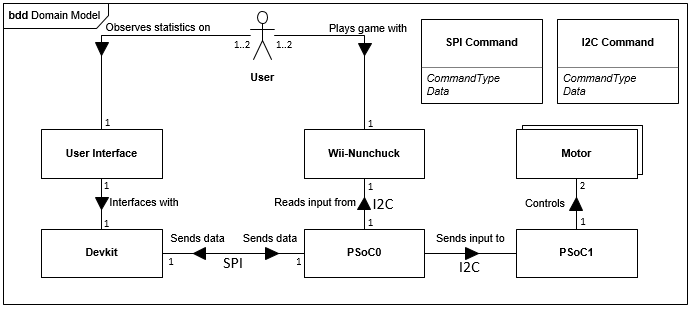
\includegraphics[width=\textwidth]{SystemArkitektur/images/DomainModel.PNG}
	\caption{Systemets domænemodel}
	\label{figure:domainModel}
\end{figure}

Her repræsenteres hardware som blokke forbundet med associeringer. Associeringerne viser grænsefladerne mellem de forbundne hardware komponenter (Enten \textit{SPI} eller \textit{I2C}), samt retningen af kommunikationen. Af modellen fremstår konceptuelle kommandoer for grænsefladerne, som beskriver deres nødvændige attributter.

\section{Software Allokering}

Domænemodellen i figur \ref{figure:allocationDiagram} præsenterer systemets hardwareblokke. På figur \ref{figure:allocationDiagram} ses et software allokeringsdiagram, som viser hvilke hardwareblokke der har softwaredele af systemet allokeret på sig. 

\begin{figure}[H]
	\centering
	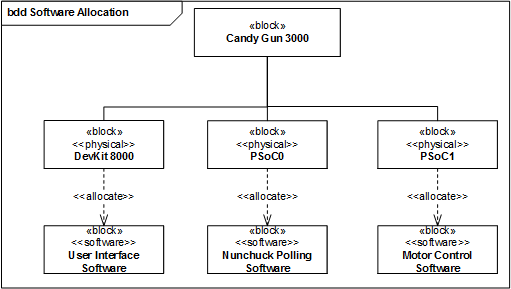
\includegraphics[width=\textwidth]{SystemArkitektur/images/SoftwareAllocation.PNG}
	\caption{Systemets software allokeringsdiagram}
	\label{figure:allocationDiagram}
\end{figure}

Det kan her ses at systemet består af tre primære softwaredele: \textit{DevKit 8000 Software}, \textit{PSoC0 Software}, \textit{PSoC1 Software}. Disse er fordelt over de 3 tilsvarende CPU'er.

\section{Hardware}

\subsection{BDD}

\subsection{IBD}

\section{Software}

\subsection{SPI Kommunikations Protokol}

\subsection{I2C Kommunikations Protokol}

\section{Signalbeskrivelse}
	\begin{tabular}{|>{\hspace{0pt}}p{1.5cm}  >{\hspace{0pt}}p{3cm} | p{2.5cm} | p{2.5cm} | p{2.5cm} |}
		\hline
		\textbf{Blok-navn} & \textbf{Funktionsbeskrivelse} & \textbf{Signaler} & \textbf{Kommentar} & 3\\ \hline
		Mål & & Klarhed om projekt idé, samt de vigtigste krav bla bla bla bla & blabla & blabla\\ \hline
		Længde & & 1 uge & 3 uger & 3 uger\\ \hline
		Disciplin & Artefakt & Inception 1 & ... & ...\\ \hline
		\textbf{Projekt Formulering} & hey hey hey hey & Udled projektformulering. Anvend MosCoW til at bla bla bla & & \\ \hline
		\textbf{\hspace{0pt}Specifikation} & Kravspecifikation \& Accepttest & ... & ... & ... \\ \hline
		\textbf{Arkitektur} & Systemarkitektur & Ingen & bla bla & bla bla \\ \hline
		\textbf{Design} & Design dokumentation & Ingen & bla bla & bla bla\\ \hline
		\textbf{Implementering og modul test} & HW/SW/Mekanik & Ingen & bla bla & bla bla \\ \hline
		\textbf{Projekt styring} & Projekt plan & bla bla & bla bla & bla bla \\ \hline
		\end{tabular}
\subsection{Specifikation og Analyse}